\chapter{Retrieval Policies, Evidence Assembly, and Grounded Execution}\label{ch:C16}

The 2026 retrieval evidence spans ReFind's controlled search over raw chat, LGM's query-conditioned latent graph, and MATM's state-conditioned procedural continuations~\cite{cumb2026refindv2,cumb2026lgmv2,kim2026matm}. Their different representation and computation boundaries prevent a single structure-based ranking. A rigorous comparison follows evidence from the stored object through access and assembly to the decision it actually changes.

\section{Retrieval selects evidence for an action}\label{sec:C16:objective}
Retrieval in an agent system is the selection of information that can change a consequential decision. The retrieved object may be a document passage, a temporal fact, a prior trajectory, a skill, or a tool description. These objects have different relevance criteria. A passage can support an answer without authorizing an action. A successful trajectory can suggest a procedure without proving that its preconditions hold now. Retrieval quality should therefore be defined relative to the decision and the role of the retrieved object.

Retrieval-augmented generation established a model in which generation conditions on external retrieved evidence~\cite{lewis2020rag}. That foundational formulation is not a description of every current agent-memory system. By the October 2026 cutoff, active graph traversal, state-conditioned trajectory retrieval, and runtime context construction make memory access a multi-step control process. The retriever and the reasoning policy can interact repeatedly rather than following a fixed retrieve-once-then-answer pipeline.

Let $S$ be the current task state, $D$ the available evidence store, and $Y$ the evaluation target. A retrieval policy $\rho$ selects $R=\rho(S,D)$ without observing $Y$. Let $\mathfrak R_A(S,D)$ contain the evidence subsets allowed by the current access policy $A$. For a fixed joint distribution of $(S,D,Y)$, a proposed objective is
\begin{equation}
 \begin{aligned}
 \min_{\rho,\pi}\quad &\mathbb E\!\left[
 \ell(a,Y)+\lambda C(\rho(S,D),S)\right],\\
 \text{subject to}\quad &\rho(S,D)\in\mathfrak R_A(S,D).
 \end{aligned}
\end{equation}
Here $a\sim\pi(\cdot\mid S,\rho(S,D))$ follows the actual deployed decoding and parsing law, and the expectation includes its randomness. The nonnegative resource cost $C$ includes search, reranking, context assembly, and generation; $\lambda\geq0$ converts that cost to the scale of the decision loss $\ell$. Missing-evidence consequences belong to the loss term. Relevance labels based on lexical overlap or passage entailment are proxies for this objective. They can be useful training targets without fully capturing whether the evidence changes the final action correctly.

The distinction matters for tool execution. An agent can retrieve the right account identifier but the wrong version of a permission policy. It can locate a valid example of an API call whose side effects differ from the present request. A retrieval metric that marks the identifier passage relevant can score the step as successful while the resulting tool call remains invalid. End-to-end evaluation should retain these roles and inspect the first decision at which the missing distinction matters.

Evidence also competes for a finite input budget. More retrieved items can increase recall while reducing the policy's ability to identify the authoritative ones. A retrieval system should report candidate recall, final evidence packing, and downstream use separately. A method that retrieves a decisive record but drops it during prompt construction has an assembly failure; a method that includes it but follows a stale conflict has an interpretation failure. Those distinctions guide different repairs.

For a specified decisive-evidence path, define nested events $E_1\supseteq E_2\supseteq E_3\supseteq E_4$: the required source is available and authorized, reaches the candidate set, survives packing with its qualification, and is appropriately used. When the conditioning events have positive probability,
\begin{equation}
 P(E_4)=P(E_1)\prod_{j=2}^{4}P(E_j\mid E_{j-1}).
\end{equation}
This is the probability chain rule, with no stage-independence assumption. It measures this evidence path, not all task success: another source or a different valid plan can bypass it. Conditional stage metrics expose a bottleneck that an aggregate recall score cannot locate. They should be estimated on the same workload cohort; multiplying rates from unrelated benchmarks is invalid. MRAgent, JAM, MATM, and MemCalib intervene at different factors, which is why their reported scores cannot be treated as interchangeable evidence of retrieval quality.



Figure~\ref{fig:C16:overview} isolates the mechanism and its stated information boundaries.
\begin{figure}[!htbp]
\centering
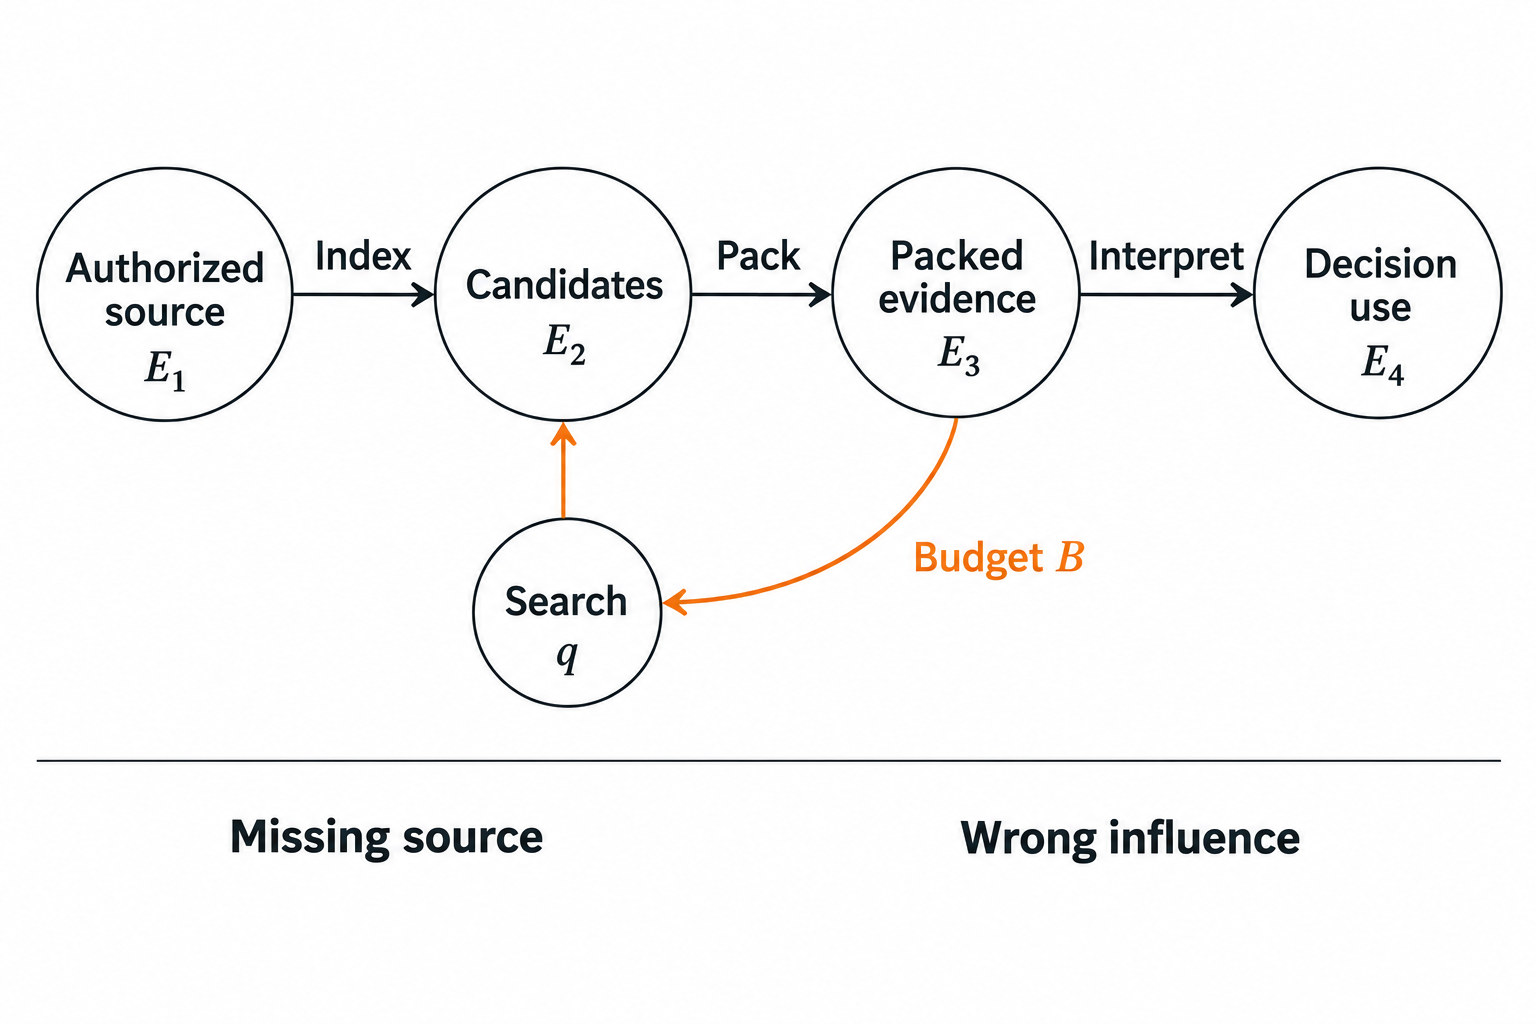
\includegraphics[width=\linewidth]{book/figures/assets/F16review.png}
\caption{A decisive-evidence path with separate failure boundaries. Authorized source availability, candidate selection, qualified packing and appropriate use are nested events for this specified path. Conditional stage probabilities multiply without an independence assumption. Alternative valid evidence paths may still solve the task. A return to search is a policy choice with cost; it does not establish evidence sufficiency.}
\label{fig:C16:overview}
\end{figure}

\section{Index units and information boundaries}\label{sec:C16:index}
The indexing unit determines which relations retrieval can preserve. Fixed token chunks are simple but can separate an assertion from its qualification, a tool call from its result, or a correction from the statement it revises. Structural units such as sections, messages, episodes, and typed records can preserve those boundaries, but they vary in length and can contain multiple propositions with different authority. Chunking is part of the representation, not a neutral preprocessing detail.

A document index should retain source identity, version, location, timestamp, and access scope. An agent-memory index additionally needs event and session relationships. If a retrieved passage is regenerated from a summary, its identifier should distinguish the summary from the original source. Otherwise a citation can appear precise while pointing to an unsupported abstraction. A hierarchy can provide compact navigational text while keeping a path to exact evidence.

Dense retrieval uses learned representations to compare queries and candidates; lexical retrieval provides a complementary signal for exact strings, identifiers, and uncommon terms. Hybrid retrieval is an engineering response to different failure modes, not a universal guarantee. Dense similarity can miss a newly introduced identifier, while lexical overlap can retrieve a misleading near-duplicate. Query construction and metadata filtering should reflect the task rather than assuming one similarity function captures every relation.

Versioned indexing is necessary when documents change. A vector for an old passage can remain searchable after the displayed text has been replaced, creating an evidence mismatch. Store an index-generation identifier and source-content digest, and reject or refresh stale results according to the application contract. Re-embedding the entire corpus can be expensive; incremental updates require careful deletion and alias handling. The cost of these operations belongs in the lifecycle boundary.

Access filtering should occur before exposing content to an unauthorized model or worker. Filtering only the final answer does not undo the disclosure. Search ranking can itself reveal sensitive metadata if unauthorized records affect returned scores or counts. A strong application contract identifies which metadata may be visible, which store partitions are isolated, and how cached results are invalidated after access changes. Retrieval is an information-flow boundary as well as a ranking stage.

The September LGM method changes the representation boundary itself. It pools selected backbone hidden states, obtains sparse concept activations through an autoencoder, constructs query-dependent graph relations, and conditions generation through learned latent prefix tokens. Its training combines response generation, evidence reconstruction, and sparse reconstruction objectives~\cite{cumb2026lgmv2}. These are coupled learned mechanisms, unlike an external text graph used only for lookup. The ``neuro-symbolic'' designation does not establish logical soundness or uniquely identifiable concepts: sparse activations and learned message passing do not by themselves prove either. A structure ablation must therefore control backbone adaptation, prefix capacity, and evidence-reconstruction supervision before assigning the full gain to graph topology. Reusing the latent bank after changing its encoder or consumer also requires the compatibility tests of Chapter~\ref{ch:C17}.

A proposed index audit samples records across document formats and update histories, checks that every returned item resolves to the recorded version, and verifies that qualification and role boundaries survive chunking. It should include deleted sources, renamed artifacts, repeated identifiers, and contradictory revisions. These checks do not prove semantic usefulness, but they establish that the retriever is searching the evidence it claims to search.


\section{Query construction and adaptive access}\label{sec:C16:adaptive}
A query is a hypothesis about which evidence will help. Query rewriting can add useful bridge concepts, but it can also encode an early mistaken interpretation and narrow the search prematurely. An adaptive agent should preserve uncertainty about its information need and revise the query when returned evidence contradicts its assumptions. The memory access policy is then part of reasoning rather than a fixed frontend.

MRAgent uses a Cue--Tag--Content graph and an active reconstruction loop~\cite{mragent2026}. Tags act as associative intermediates, allowing the model to select relations and then fetch content rather than expanding every neighboring node. The mechanism can use newly discovered cues to change later traversal. Its theoretical separation from restricted passive retrieval depends on the constructed task family and access assumptions; it should not be interpreted as a proof that every active agent outperforms every static retriever. Its published code provides a concrete object for implementation inspection.

JAM separates a hierarchical store retaining raw histories from a runtime Researcher that uses search, open, and browse actions to assemble query-specific context~\cite{jit2026research}. Its training combines verified-trajectory supervision with a subsequent policy-optimization stage. This changes the accounting boundary: less irreversible preprocessing can preserve details, while runtime exploration introduces model calls and latency. Query-conditioned construction does not remove the need for retention, access controls, or calibrated stopping when evidence remains incomplete.

The two mechanisms differ in what is navigated. MRAgent traverses explicit associative relations; JAM navigates a hierarchical workspace with raw pages and summaries. A clean comparison would hold raw evidence, model, maximum accessed content, and total compute fixed while varying the access representation. Without that control, an improvement can arise from more evidence, more reasoning calls, a different training distribution, or a better interface. The architecture's name does not identify the cause.

Adaptive access requires a stopping rule. Let $b$ be the current evidence state and let $a$ be a possible retrieval action. An ideal controller would choose an action when its expected reduction in task loss exceeds its cost. In practice that value is uncertain, and self-assessed sufficiency can be overconfident. A useful implementation distinguishes stopping because evidence is sufficient from stopping because the budget is exhausted. Both can produce an answer, but only the first asserts that the information requirement was met.

A bounded decision model clarifies that stopping rule. Let $\xi\in\Xi$ be a sufficient controlled query state, including the target belief, query-use/history information, source/interface versions and permissions needed to determine available queries, costs, observation kernels and future state. Its target-belief projection is $b_\xi=\Pr(Y\in\cdot\mid\xi)$ for a fixed target $Y$. A posterior over $Y$ alone need not be sufficient: identical target probabilities can coexist with different remaining queries or observation laws. For a fixed finite legitimate action set $\mathcal A$ and loss $\ell:\mathcal A\times\mathcal Y\to[0,L_{\max}]$ with finite $L_{\max}$, set $\mathcal R(b)=\min_{a\in\mathcal A}\mathbb E_b\ell(a,Y)$. A permitted read-only query $q$ has observation kernel $K(\mathrm d o\mid\xi,q)$ and sufficient-state update $T(\xi,q,o)$. Assume Bayes-consistent target posteriors and that query selection uses only $\xi$ and independent randomization, so selection itself supplies no hidden target information. Its one-step information value is
\begin{equation}
 V_q(\xi)=\mathcal R(b_\xi)-
 \mathbb E_{o\mid\xi,q}\mathcal R(b_{T(\xi,q,o)})\geq0.
\end{equation}
The inequality holds because the decision maker may ignore the new observation and retain its former rule. It does not describe a fallible deployed model, which may be distracted or misled by the returned text. It also does not compare different authority sets or changed task objectives.

Let $\mathcal Q(\xi)$ be a finite available query family, $B\geq0$ a finite resource budget, $c(\xi,q)\geq0$ the declared query cost, and $\lambda\geq0$ a finite loss-scale multiplier. Write $\mathcal Q_B(\xi)=\{q\in\mathcal Q(\xi):c(\xi,q)\leq B\}$. An explicit remaining-query horizon $n\in\mathbb N_0$ gives the finite-horizon controller
\begin{equation}
\begin{aligned}
 W_0(\xi,B)&=\mathcal R(b_\xi),\\
 D_n(\xi,B,q)&=\lambda c(\xi,q)+\mathbb E_{o\mid\xi,q}
 W_{n-1}(T(\xi,q,o),B-c(\xi,q)),\\
 W_n(\xi,B)&=\min\!\left\{\mathcal R(b_\xi),
 \min_{q\in\mathcal Q_B(\xi)}D_n(\xi,B,q)\right\},\quad n\geq1.
\end{aligned}
\end{equation}
With no feasible query the inner minimum is $+\infty$. Unavailable results remain observations with incurred cost. The explicit horizon terminates the recursion even when a permitted query has zero modeled cost. A budget alone bounds query count only under an additional positive lower cost bound. A myopic comparison $V_q(\xi)>\lambda c(\xi,q)$ can miss complementary multi-query evidence; the recursion exposes that limitation without claiming that a correct sufficient state or observation model is available in a production agent. Log budget or horizon exhaustion separately from a verified evidence-sufficiency decision.

The proposed diagnostic logs each information need, query, selected relation or page, returned evidence, and reason for stopping. It then replays failed cases with an oracle bridge cue or a missing page supplied. Repair under that intervention supports an access-policy bottleneck. Failure despite the evidence shifts attention to interpretation or action selection. This analysis is more informative than counting how many search calls an agent made.

The released code makes several boundaries more concrete. In the inspected MRAgent \path{Agent.answer_question} path, question-key extraction precedes graph-relation evaluation; temporal questions can take a specialized branch, and non-temporal evidence undergoes coarse selection, identifier-based deduplication, finer selection, and key-tag expansion before the tool-enabled answer stage~\cite{repo_mragent2026}. These operations mean that a graph match is not identical to final evidence exposure. Deduplication by identifier prefix can reduce repeated material while also changing how much supporting detail survives. A reproduction should log both pre-selection candidates and the final answer input.

The repository linked by JAM includes a research implementation whose \texttt{ResearchAgent.research} refreshes retrievers, loads memory, plans a search, accumulates a temporary result, and reflects on sufficiency~\cite{repo_jam2026}. It records iterations and stops either when the reflection says enough or when the configured iteration bound ends. The returned integrated memory alone does not distinguish those stopping causes; the raw iteration record is needed to reconstruct them. The inspected March 2026 repository revision precedes the September JAM report. Its research and application variants therefore do not, by themselves, establish the deployed weights, training path, or every runtime interface of the paper's trained configuration. Public code and paper mechanism must be mapped at that narrower boundary.

MATM's inspected \texttt{UnifiedRerankerOrchestrator.rerank} supports staged reranking, normalizes candidates into one schema, and retains stage-level error metadata~\cite{repo_matm2026}. In the inspected error path, a failed stage can preserve its upstream candidate order instead of producing a new ranking. Thus a run configured for learned reranking need not actually apply that ranking on every query. Reporting configured mode without stage application and error counters can misattribute a result to the reranker. These are source observations at pinned revisions, not measured error frequencies or reproduced benchmark outcomes.


\section{State-conditioned procedural retrieval}\label{sec:C16:trajectories}
Procedural retrieval should match the consumer's current situation rather than only the initial task description. Multi-Agent Transactive Memory indexes recent observation-action context as a key and a subsequent continuation as its value, enabling one agent to reuse another agent's experience~\cite{kim2026matm}. A learned reranker estimates downstream utility beyond initial similarity. The method concerns shared artifacts across heterogeneous agents; it does not require that the agents jointly train or communicate during each task.

The essential indexing boundary is temporal. A key must contain information available before the continuation begins; the value can contain the later actions offered as guidance. If a key accidentally includes the successful future result, retrieval can exploit information unavailable to a real consumer. This is a procedural form of leakage. Dataset construction should validate the cutoff at each indexed step and preserve environment boundaries when sliding windows are formed.

The reported ALFWorld comparison improves from 47.08\% without memory to 64.31\% with retrieval and learned reranking, while WebArena gains are smaller~\cite{kim2026matm}. These are author-reported population results under the paper's allocations and environments, not a universal memory-system ranking. Generating the experience repository and training rerankers also consume resources. Consumer-side savings should not be described as total lifecycle savings unless those production costs are included or explicitly amortized.

An executable continuation is not a command to replay blindly. A different consumer may have a different tool set, current object state, or authorization. The retrieved trajectory should be treated as evidence for a candidate plan whose preconditions must be checked. A replay mechanism that substitutes identifiers from the current task can still preserve a hidden assumption from the producer's environment. The interface should expose those assumptions where possible and allow abstention or fresh exploration.

HyperSkill's subtask and task routes provide a contrasting procedural index~\cite{xu2026hyperskill}. Rather than supplying only a raw continuation, they retrieve lessons and skills associated with relevant trajectories. This can improve abstraction and reduce raw context, while introducing extraction and consolidation error. MATM and HyperSkill therefore compare along representation, timing, feedback, and cost axes. An aggregate success difference without matched consumer and producer budgets would not isolate whether raw or abstract experience is the better transferable object.

The proposed evaluation separates near-duplicate reuse, compositional transfer, and cross-environment transfer. Near-duplicate retrieval tests useful caching but is weak evidence for general procedural learning. Compositional transfer holds out combinations of known subtasks. Cross-environment transfer changes tools or state dynamics and tests compatibility. Report all three rather than pooling them into one ``generalization'' score.


\section{Evidence packing attribution and influence}\label{sec:C16:packing}
Retrieved content becomes useful only after it reaches the model in an interpretable form. Packing determines ordering, redundancy, source labels, and the separation between evidence and instruction. A strong ranker can still fail if the prompt truncates its best result or strips the qualification that made it relevant. The packed context should be treated as a versioned artifact that can be reconstructed for audit.

MemCalib studies a downstream distinction: a memory atom can be appropriately ignored, provide bounded support, or control a material conclusion~\cite{memcalib2026}. Its benchmark supplies composite memory blocks and annotates intended influence at the atomic level. Its training method separates overuse and underuse signals and redistributes credit using counterfactual localization. These results evaluate use of supplied memory, not the quality of a complete storage-and-retrieval system. The distinction limits the claim while making the post-retrieval problem experimentally visible.

Influence should follow role and authority. A product page can provide a claimed feature, a paper can provide an author-reported result, and a user message can provide a task constraint. Packing all three as equally authoritative text invites category errors. The model-visible representation should preserve source type and scope. It should also mark deductions separately from observations so that later summarization does not promote a proposed explanation into cited evidence.

Attribution requires a mapping from an output claim or action to supporting evidence. For a text answer, this can be a claim-span-to-source relation. For tool execution, it can include the source of each argument and the authority permitting its effect. A citation to a long document is not sufficient when the cited passage does not entail the claim. Source availability, source relevance, and claim support are different checks.

Conflicting evidence should remain visible until resolved. A packer that chooses only the highest-scoring passage can erase a known disagreement and create false certainty. A proposed packing objective reserves space for support, relevant contradiction, and unresolved uncertainty. This can reduce the number of distinct positive passages that fit, so its value should be evaluated through decision correctness and calibration rather than raw recall. The best evidence set can contain a passage that argues against the tentative answer.

The implementation should log both retrieved candidates and the final injected set. Record which records were excluded for budget, access, duplication, staleness, or low relevance. This supports targeted failure analysis and prevents a system from claiming that a fact was ``retrieved'' merely because it appeared in an internal candidate list. The final conditional input is the evidence boundary that matters for the policy.


\section{A worked multi-step evidence dependency}\label{sec:C16:worked}
Consider a research agent asked whether a newly announced system improves long-horizon reliability. One source is a product announcement, another is an earlier technical report, and a third is a revised paper whose evaluation changes the reported gain. A whole-query embedding may rank the announcement first because it repeats the system name and the phrase ``long-horizon.'' The decisive evidence instead requires identifying the version lineage, the evaluation metric, and whether the tasks match the stated reliability claim.

A suitable evidence plan separates these needs. First resolve the canonical identity and versions. Next retrieve the method and evaluation protocol. Then locate the result table and limitations. Finally compare whether ``reliability'' means mean success, all-repeated-runs success, or a best-of-many metric. This is a constructed example, not a claim about a particular named system. It shows how retrieval targets can depend on earlier findings instead of being fully specified by the original query.

Represent the dependency as a directed acyclic graph of evidence requirements: identity precedes version-specific result selection; metric definition precedes interpretation; task distribution precedes transfer claims. The graph is a planning aid rather than a world model. A node can be unresolved, supported, contradicted, or unavailable. Reaching a final answer while an essential node remains unresolved should produce a qualified conclusion rather than a fabricated bridge.

Suppose the first retrieved result reports any-of-five success and the revised paper reports repeated-run reliability on a different split. Subtracting the two percentages would be invalid even if both were copied perfectly. Retrieval accuracy cannot repair a comparison-axis error. The synthesis stage must align attempts, denominators, splits, backbones, and budgets before ranking methods. A structured evidence table is often more reliable than a generated prose comparison because it makes missing fields explicit.

The proposed counterfactual test removes one requirement at a time. Hide the revision notice, hide the metric definition, or replace the primary report with a secondary summary. Observe which claim changes and whether the agent detects the missing dependency. A successful system should be able to revise its conclusion after new evidence arrives without discarding unrelated valid findings. This measures evidence integration and update behavior, not merely answer recall.

The same structure applies to execution. Before a tool action, the agent may need an object identifier, current resource version, relevant constraint, and authorization. These can come from different sources and have different freshness requirements. Grounded execution therefore extends retrieval beyond document question answering: it assembles a justified action under current state and authority, with the supporting evidence preserved in the run record.


\section{Evaluation contamination and uncertainty}\label{sec:C16:evaluation}
A retrieval evaluation should specify the unit of relevance and the unit of success. Passage relevance can be judged independently of answer generation, while task success includes retrieval, reasoning, and execution. Report both when possible. An oracle evidence condition identifies a useful ceiling, but it must be labeled as diagnostic because a real system does not know the decisive evidence in advance.

ReFind supplies a concrete counterweight to assuming that more elaborate memory structure is necessarily better. It retains raw chat turns, uses lexical indexing, and gives an iterative agent controls for session-aware rank fusion, neighborhood expansion, time filtering, and previously inspected sessions; a separate stage answers from saved evidence~\cite{cumb2026refindv2}. The absence of generated semantic structure does not mean the absence of organization: session boundaries and timestamps remain essential. Its reused leaderboard baselines should be distinguished from its matched control experiments. The scientific comparison is thus not ``raw versus structured'' in isolation, but offline abstraction versus query-time search under specified access controls, backbone, final evidence, and complete cost. This baseline is especially relevant before attributing gains to a graph or to expensive LLM-based index construction.

Use retrieval ablations that preserve final context length. Comparing a graph method returning many rich records with a flat baseline returning fewer tokens confounds structure and evidence volume. Similarly, comparing an active retriever with a one-shot baseline under equal retrieval-call limits can conceal additional model computation. Match either complete resource budgets or report a Pareto surface over success, token use, tool interactions, latency, and construction cost. One scalar rank rarely captures all relevant tradeoffs.

Contamination can enter through the index, training data, task generator, and reranker labels. A trajectory index containing near-duplicate evaluation solutions can create a useful reuse system while weakening a claim of novel-task reasoning. Separate the producer and consumer splits, record artifact timestamps, and audit duplicate or templated trajectories. If synthetic queries are generated from known evidence, evaluate whether their wording makes the source unusually easy to retrieve.

Longitudinal stores introduce order dependence. A task can become easier because a previous evaluation task inserted its answer into memory. This may be an intended continual-learning setting, but it is not equivalent to an independent held-out test. Declare whether updates are allowed, reset stores between conditions where required, and report frozen-index and evolving-index results separately. Paired direct and indirect questions should read the same frozen state when the goal is to diagnose implicit relevance.

Uncertainty should include tasks, corpus samples, and stochastic access policies. Repeating decoding on a single fixed corpus does not estimate robustness to document composition. Rebuilding an index with a different embedding model can change candidate sets and calibration, not just vector quality. Treat index generation as part of the configuration. Judge-based relevance and citation scoring should be checked against an independently reviewed subset, with disagreement retained.

None of the proposed evaluations has been run for this monograph. The reviewed 2026 methods provide concrete mechanisms and author-reported evidence under their stated settings. A rigorous survey can compare those mechanisms, identify causal confounds, and derive discriminating tests without presenting new measurements. That boundary is especially important when active retrieval is advertised as a general solution to memory: its benefits remain conditional on what was stored, how it was indexed, and what the policy can infer.


\section{An execution contract for grounded retrieval}\label{sec:C16:contract}
A proposed grounded-retrieval contract has six stages: define the information need, enforce access, retrieve candidates, verify source/version identity, assemble evidence with roles, and validate the resulting claim or action. Each stage emits inspectable artifacts. The contract is not a universal algorithm and does not guarantee that a model reasons correctly. It specifies the interfaces at which errors and unsupported transitions can be detected.

For execution, augment the evidence packet with freshness requirements and a precondition check. A retrieved resource state may have changed between search and tool dispatch. If the action depends on that state, revalidate it or use a conditional write supported by the remote service. Retrieval confidence cannot substitute for concurrency control. A perfect passage about an old state can justify the wrong present action.

Index compression and evidence compression should be audited separately. A fixed-dimensional document vector can discard the distinction needed to select a source, while a later passage packer can discard that distinction after the correct source was selected. Increasing the generation window repairs neither failure automatically. In a constructed diagnostic, first supply the correct document identifier while preserving the ordinary passage selector; then supply the decisive passage while preserving the ordinary packer. The two interventions locate losses at different boundaries. They are oracle diagnostic conditions, not deployable baselines. Account for the document-search, passage-scoring, and generation costs independently, and retain the final evidence spans so that the apparent benefit of a larger index cannot be confused with a larger model-visible evidence budget.

For scientific synthesis, retain the distinction among author-reported results, independently reproduced results, deductions, and proposed experiments. A retrieved repository can establish that code exists at a commit; it does not establish that its published experiments reproduce. An official product document can establish a documented interface; it does not reveal every proprietary implementation decision. The output should carry the same evidence boundary that the source supports.

Current 2026 retrieval mechanisms demonstrate several directions: query-conditioned runtime construction, associative traversal, shared procedural continuations, and calibrated influence of retrieved atoms. They solve different parts of the chain. JAM's preserved raw pages address pre-query information loss, MRAgent's active access addresses search adaptation, MATM's state keys address procedural matching, and MemCalib addresses use after evidence is supplied. Combining them is a design hypothesis, not an established composite result.

The original synthesis is to view retrieval as a controlled transition from stored evidence to active decision state. The transition must preserve source identity, role, time, and access scope as well as content. Its success is measured by justified behavior under bounded cost, not by the number of records returned. Chapter~\ref{ch:C17} places this transition within a unified consistency model linking the stored history, assembled context, policy, tools, and environment.

